\documentclass[times, utf8, diplomski]{fer}
\usepackage{booktabs}
\usepackage{color}
\usepackage{listings}
\usepackage{pdfpages}

\lstset{ %
language=C++,                % choose the language of the code
basicstyle=\footnotesize,       % the size of the fonts that are used for the code
numbers=left,                   % where to put the line-numbers
numberstyle=\footnotesize,      % the size of the fonts that are used for the line-numbers
stepnumber=1,                   % the step between two line-numbers. If it is 1 each line will be numbered
numbersep=5pt,                  % how far the line-numbers are from the code
backgroundcolor=\color{white},  % choose the background color. You must add \usepackage{color}
showspaces=false,               % show spaces adding particular underscores
showstringspaces=false,         % underline spaces within strings
showtabs=false,                 % show tabs within strings adding particular underscores
frame=single,           % adds a frame around the code
tabsize=2,          % sets default tabsize to 2 spaces
captionpos=b,           % sets the caption-position to bottom
breaklines=true,        % sets automatic line breaking
breakatwhitespace=false,    % sets if automatic breaks should only happen at whitespace
escapeinside={\%*}{*)}          % if you want to add a comment within your code
}

\begin{document}

% TODO: Navedite broj rada.
\thesisnumber{2926}

% TODO: Navedite naslov rada.
\title{3D interaktivna vizualizacija simulacije vibracija}

\author{Nikola Vugdelija}

\maketitle

% Ispis stranice s napomenom o umetanju izvornika rada.
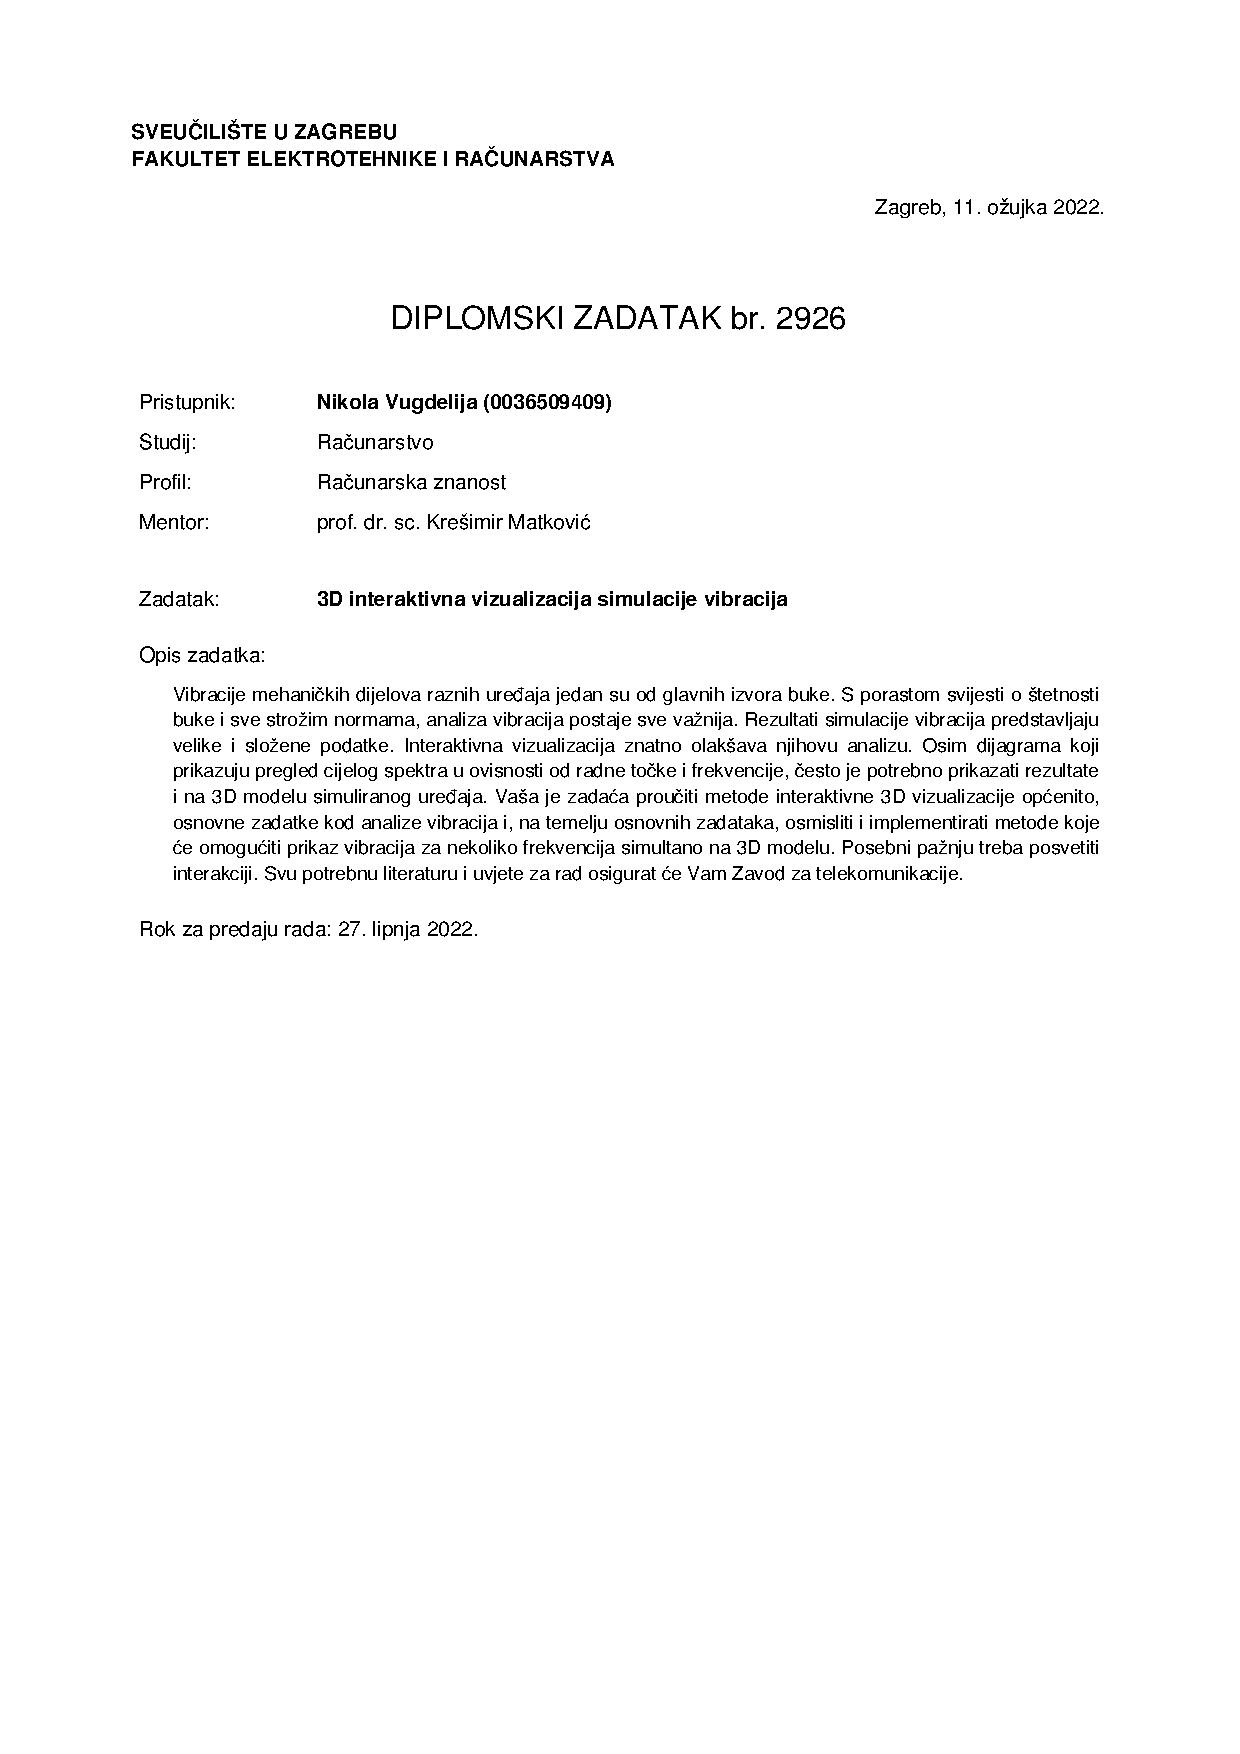
\includepdf[pages=-]{resources/docs/task.pdf}


% Dodavanje zahvale ili prazne stranice. Ako ne želite dodati zahvalu, naredbu ostavite radi prazne stranice.
\zahvala{Bogu hvala!}

\tableofcontents

\listoffigures

\chapter{Uvod}
Buka i vibriranje motora su jedni od ključnih faktora koji utječu na osjećaj udobnosti putnika u osobnom automobilu. No, iako se može reći kako je osjećaj udobnosti subjektivne prirode, propisi koji kontroliraju dozvoljene razine buke motora vozila pri određenim brzinama su objektivni i egzaktni. Zbog navedenih razloga je inženjerima iznimno važno da je vibriranje motora prilikom rada na što nižoj razini, a najjednostavniji način na koji to mogu provjeriti u fazi projektiranja motora je pomoću NVH \engl{Noise, Vibration, Harshness} simulacija. NVH simulacije inženjerima omogućuju precizan uvid u razinu vibriranja pojedinih dijelova motora, a probleme koji mogu uzrokovati vibraciju mogu rješavati prilikom projektiranja.\\
No, računanje simulacije je samo dio problema. Računske simulacije ove vrste, nerijetko proizvode podatke koje se ne može jednostavno vizualizirati i analizirati \citep{matkovic2021getting}. Kako bi stručnjaci mogli navedene podatke koristiti na što efikasniji način, potrebno ih je intuitivno i razumljivo prikazati. Iako su podaci koji su prikazani u obliku tablica i grafova korisni, vizualizacijom istih podataka na 3D modelu motora se postiže jasniji, intuitivniji i potpuniji prikaz rada motora.\\
Ovaj rad opisuje izradu alata za vizualizaciju podataka dobivenih iz NVH simulacije pomoću 3D modela motora i 2D grafova. Fokus predstavljenog alata je na vizualizaciji vibracija motora prilikom rada na višestrukom broju frekvencija, kako bi se razine vibracije različitih taktova motora jednostavnije uspoređivale.

\chapter{Pregled područja}
Iako često zanemarena, vizualizacija podataka je iznimno važno područje analize podataka. Pošto isti skup podataka može prenijeti potpuno drugačije informacije ovisno o načinu prikaza, od velike je važnosti odabrati optimalne vizualizacijske tehnike za konkretni skup podataka. Ali kako je naglašeno u \citep{Unwin2020Why}, kod vizualizacije ne postoji jedna, "optimalna" grafika koja vrijedi za svaki skup podataka, nego je često potrebno pronaći grupu vizualizacijskih tehnika koje se međusobno upotpunjuju i prikazuju cjelovitu sliku. Stoga je tijekom osmišljavanja alata za vizualizaciju izrazito važno utvrditi za koju svrhu se taj alat koristi, te koje informacije je potrebno njime vizualizirati iz danog skupa podataka. Odgovori na navedena pitanja postaju kompleksniji za odgonetnuti s porastom kompleksnosti skupa podataka koji alat vizualizira. Zbog toga je pomoć stručnjaka u domeni itekako korisna.\\
Kao što je već spomenuto, glavna svrha alata razvijenog u sklopu ovog rada je vizualizacija NVH podataka na modelu motora. Prilikom izrade ovog rada je korišten isti skup podataka koji je korišten kod \citep{matkovic2021getting}. Spomenuti podaci su izračunati NVH simulacijom pomoću alata AVL EXCITE™\citep{avlEXCITE}. Motor je zadan kao skup ćelija, a za svaku ćeliju su poznate koordinate okolnih točaka u 3D prostoru, te kojom snagom ćelija vibrira pri različitim frekvencijama rada.\\
Kako je spomenuto u \citep{matkovic2021getting}, stručnjake pri analizi NVH podataka ponajprije zanimaju tri stavke:

\begin{itemize}
\item Usporedba podataka na različitim frekvencijama rada
	\begin{itemize}
	\item Kako se vibracije mijenjaju sa promjenom frekvencije rada motora?
	\end{itemize} 
\item Lokalizacija značajki
	\begin{itemize}
	\item Koje ćelije motora pri zadanoj frekvenciji vibriraju iznosom koji pripada zadanom rasponu?
	\end{itemize} 
\item Lokalna pretraga
	\begin{itemize}
	\item Kojom snagom vibriraju odabrane ćelije?
	\end{itemize} 
\end{itemize}

Alat razvijen u \citep{matkovic2021getting} dobro adresira navedene značajke. Koristeći paralelne koordinate, omogućen je detaljan pregled usporedbe podataka na različitim frekvencijama. Adresiranje druge i treće značajke je olakšano omogućavanjem korištenja višestrukih, međusobno povezanih prozora sa 3D prikazom motora. Lokalna pretraga je ostvarena uz pomoć "kista" kojim korisnik može odabrati raspon iznosa za određene frekvencije, a svi prozori automatski ažuriraju prikaz modela motora označujući ćelije koje pripadaju zadanim rasponima. Konačno, u \citep{matkovic2021getting} je lokalna pretraga omogućena bojanjem modela motora bazirano na vrijednostima vibracija pojedinačnih ćelija pri radu na zadanoj frekvenciji. Detaljniji uvid u snagu vibriranja pojedine ćelije modela je omogućen odabirom interesne ćelije, nakon čega se istakne 2D graf vibracija  zadane ćelije.\\
No, iako je referirani rad cjelokupno odlično pokrio sve tri značajke, u području usporedbe podataka na različitim frekvencijama rada još ima prostora za napredak. Naime, trenutna usporedba podataka na različitim frekvencijama je moguća samo pomoću 2D grafova, koji iako korisni, imaju problema sa čitljivošću i jasnoćom. Alat koji je razvijen u sklopu ovog rada implementira niz vizualizacijskih tehnika koje potencijalno povećavaju intuitivnost usporedbe vibracija motora na različitim frekvencijama u odnosu na izvedbu kod \citep{matkovic2021getting}.

\chapter{Analiza zadatka i zahtjeva}
Pošto dizajniranje alata za vizualizaciju nije jednostavan zadatak, potrebno je poduzeti određene predprodukcijske korake kako bi se osigurala zadovoljavajuća implementacija glavnog zadatka. Navedeni je zadatak potrebno dodatno analizirati, čime bi se uočili zahtjevi potrebni za njegovo uspješno odrađivanje. Identificirane zahtjeve je također potrebno analizirati, kako bi se utvrdila njihova povezanost sa glavnim zadatkom, te osiguralo njihovo uspješno i cjelovito zadovoljavanje. 

\section{Identificirani zadaci}
Ključni zadatak alata razvijenog u sklopu ovog rada je prikazivanje razlika i sličnosti između različith frekvencija rada ćelija motora na intuitivan i razumljiv način. Kao što je već navedeno u prethodnom poglavlju, alat iz \citep{matkovic2021getting} ima problema sa čitljivošću i jasnoćom usporedbe. Usporedba utjecaja više frekvencija rada motora na vibraciju ćelija je jedino moguća koristeći grafove kod kojih svaka linija predstavlja funkciju vibracije jedne ćelije (x-os predstavlja sve frekvencije za koje postoje podaci, a y-os predstavlja snagu vibracije). Takav način rada stvara nezanemarive poteškoće sa korištenjem alata: teže je usporediti frekvencije koje nisu susjedne na grafu, čitljivost grafa je uvelike smanjena kada je odabrano više ćelija i otežano je uočiti gdje se točno na modelu motora nalaze razlike u radu motora.

\section{Identificirani zahtjevi}
Kako bi se usporedbu učinilo intuitivnijom i jasnijom, očiti korak je omogućiti iscrtavanje rezultata usporedbe na 3D modelu motora. Naime, iako se u \citep{matkovic2021getting} ćelije bojaju na temelju jačine vibracija pri radu na zadanoj frekvenciji, nije moguće iscrtati utjecaj više frekvencija na modelu motora. Takvim iscrtavanjem bi se uveliko olakšalo uočavanje promjena na dijelovima motora. Naravno, kod više odabranih frekvencija, postavlja se pitanje kako iz niza vibracija kojim ćelija vibrira pri odabranim frekvencijama, odabrati jedan konačni iznos koji će pomoću zadanog raspona i gradijenta odrediti konačnu boju ćelije kojoj pripada. Alat razvijen u sklopu ovog rada korisniku nudi nekoliko funkcija koje može odabrati, a koje primaju niz iznosa vibracija te vraćaju jednu vrijednost vibracije, koja predstavlja "sažetak" navedenog niza:

\begin{itemize}
\item MIN - najmanji iznos vibracije
\item MAX - najveći iznos 
\item AVERAGE - prosjek vibracija
\item MEDIAN - medijan vibracije
\item SPREAD - razlika između najvećeg i najmanjeg iznosa vibracije\\
\end{itemize}
Korisnik zatim može odabrati funkciju koja najbolje odgovara njegovim potrebama. Na primjer, ako korisnik treba saznati maksimalno opterećenje za svaku ćeliju pri odabiru različitih frekvencija za to mu može koristiti funkcija MAX, a ako ga zanima kolike će vibriranje ćelija varirati tijekom rada na višestrukim frekvencijama može koristiti funkciju SPREAD itd.
\\
No, kada navedene funkcije izračunaju konačnu vrijednost iz niza vrijednosti, taj iznos treba prebaciti u interval [0, 1] kako bi se omogućilo uzorkovanje gradijenta. Za ostvarivanje prijelaza u taj interval potrebno je znati koji broj označava najmanju vrijednost intervala, odnosno 0, a koji broj označava najveću vrijednost intervala, odnosno 1.
\\U alatu su ponuđena tri načina računanja navedenog raspona:

\begin{itemize}
\item GLOBAL - donju i gornju granicu raspona čine najmanji i najveći iznos vibriranja kojim neka ćelija može vibrirati tijekom rada na bilo kojoj od mogućih frekvencija
\item LOCAL - donju i gornju granicu raspona čine najmanji i najveći iznos vibriranja kojim neka ćelija može vibrirati tijekom rada na bilo kojoj od odabranih frekvencija
\item USER DEFINED - korisnik sam definira donju i gornju granicu raspona\\
\end{itemize}

Alat korisniku omogućuje da sam definira boje gradijenta na temelju kojeg će se model odrediti boje ćelija.

U sklopu alata je implementiran još jedan način "bojanja" modela motora nazvan \textit{limits mode}. Navedeni način rada baziran je na definiranim ograničenjima vibracija koja raspon vibracija dijele na 3 zone: bezopasnu, rizičnu i opasnu. Rasponi su definirani za određene frekvencije(ne nužno za sve) u posebnoj datoteci. Ovaj način bojanja je odvojen od "običnog" načina rada koji je objašnjen u prijašnjem odlomku. 
\\
Boje ćelija u \textit{limits mode}-u se određuju na sljedeći način:
\begin{itemize}
\item Zelena - ako se snage vibracije svih odabranih frekvencija za trenutnu ćeliju nalaze u bezopasnoj zoni
\item Gradijent žute - ako se snage vibracije barem jedne odabrane frekvencije nalaze u rizičnoj zoni, a nijedna u opasnoj zoni
\item Gradijent crvene - ako se snage vibracije barem jedne odabrane frekvencije nalaze u opasnoj zoni\\
\end{itemize}
Navedeni gradijenti se uzorkuju pomoću omjera broja frekvencija čiji iznos spada u zonu gradijenta i ukupnog broj odabranih frekvencija. Navedena boja i gradijenti su početno postavljeni na spomenute vrijednosti, a korisnik ih može mijenjati kako njemu odgovara.\\
Kako bi se adresirao problem sa uspoređivanjem nesusjednih frekvencija, na grafu se iscrtavaju samo podaci za odabrane frekvencije.\\
Konačno, kako bi se poboljšala čitljivost grafa u sklopu alata su implementirana dva načina iscrtavanja podataka: stupčasti i linijski, te tri načina uspoređivanja:
\begin{itemize}
\item NORMAL - svi grafovi su prikazani unutar jednog prikaza(?)
\item SUBPLOTS - svaki graf je prikazan unutar zasebnog prikaza
\item RELATIVE - kao NORMAL, ali je dodatno moguće odabrati jednu ćeliju s obzirom na koju će se prikazati grafovi svih ostalih ćelija\\
\end{itemize}
Navedeno rješenje predstavlja poboljšanje na području čitljivosti zbog više razloga. Više nisu grafovi svih ćelija prikazani odjednom, već su samo prikazani grafovi odabranih ćelija. Moguće je prikazati svaki graf na zasebnom prikazu, čime je pojednostavljeno uspoređivanje u slučaju više odabranih ćelija. Sa relativnim uspoređivanjem, korisnik može lakše usporediti odabranu ćeliju sa ostalim ćelijama. Konačno, pošto su omogućena dva načina iscrtavanja podataka, korisnik može odabrati onaj način koji odgovara njegovim potrebama i preferencama, te nije prisiljen koristiti linije za iscrtavanje grafova.

\chapter{Dizajn vizualizacije}

Zahtjevi navedeni u prijašnjem poglavlju daju naslutiti kako će sučelje alata biti kompleksno, pošto brojne opcije korisniku trebaju biti na raspolaganju. Kako bi se svi navedeni zahtjevi zadovoljili, a upotrebljivost alata se ne bi smanjila, potrebno je alat organizirati u smislene prikaze \engl{view}. Na slici \ref{fig:gen-screen} se može vidjeti kako je alat zapravo organiziran u sedam prikaza. Navedeni prikazi su detaljno opisani u nastavku.\\

\begin{figure}[htb]
\centering
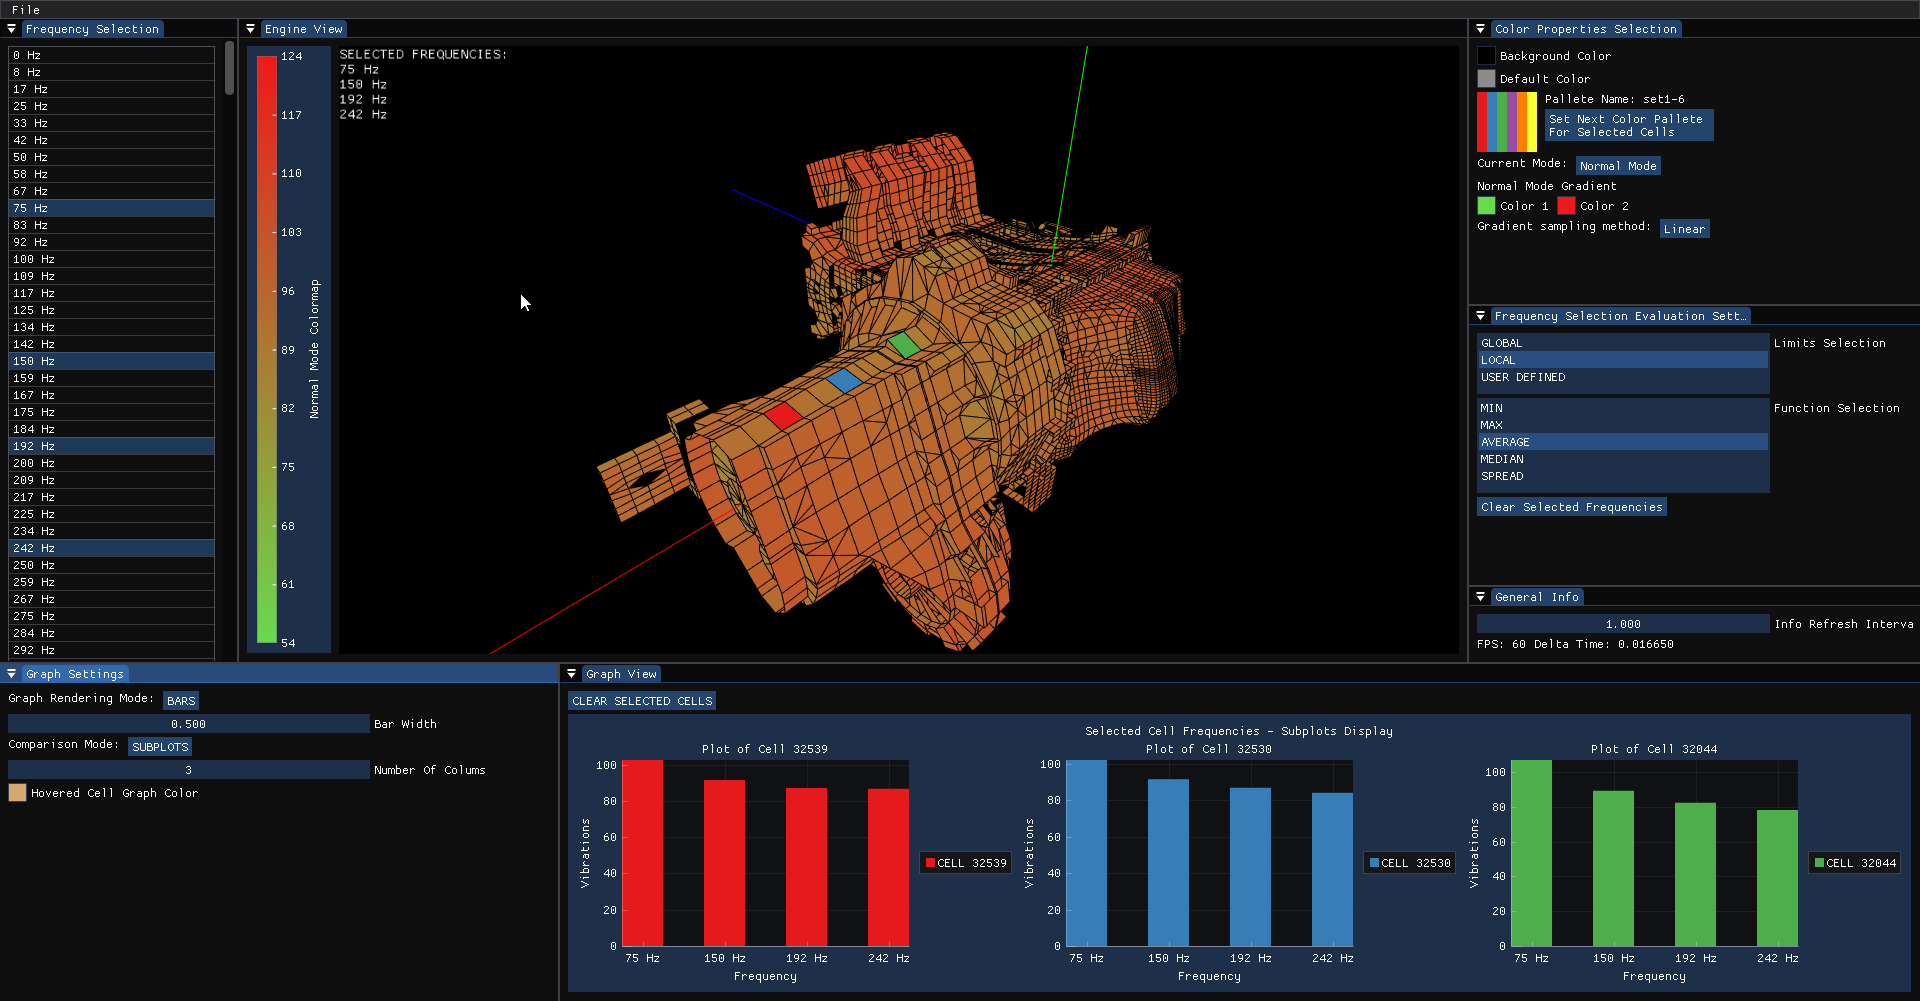
\includegraphics[width=15cm]{resources/images/general_screenshot.png}
\caption{Snimka zaslona alata}
\label{fig:gen-screen}
\end{figure}


\section{Prikaz motora}

\section{Prikaz grafa}

\section{Postavke grafa}

\section{Odabir frekvencija}

\section{Postavke evaluacije odabranih frekvencija}

\section{Postavke boja}

\section{Generalne informacije}


\chapter{Implementacija}

\begin{lstlisting}
//ovdje
\end{lstlisting}

\chapter{Demonstracija rada alata}
Par sličica i tako to.

\chapter{Zaključak}
Zaključak.

\bibliography{literatura}
\bibliographystyle{fer}

\begin{sazetak}
Sažetak na hrvatskom jeziku.

\kljucnerijeci{Ključne riječi, odvojene zarezima.}
\end{sazetak}

% TODO: Navedite naslov na engleskom jeziku.
\engtitle{3D Interactive Visualization of Vibration Simulation}
\begin{abstract}
Abstract.

\keywords{Keywords.}
\end{abstract}

\end{document}
